% Tutorial 06

\subsection{Tutorial 6: NN(QM)/MM simulations with the BuRNN approach}

The Buffer Region Neural Network (BuRNN) approach \cite{Lier2022BuRNN} is a hybrid quantum mechanics/molecular mechanics (QM/MM) \cite{Warshel1976QM/MM, Senn2009QM/MM} simulation method. The system is therefore partitioned into regions having different levels of theory, a QM (inner) and a classical MM (outer) region. 

In-between the two regions an additional buffer region is introduced to be treated at both levels of theory (Figure~\ref{BuRNN_scheme}, a). The inner region and the interactions between the inner region and the buffer region are described by an atomistic neural network (NN) model.

The total potential energy of the system is calculated as follows:

\begin{equation}
  \begin{aligned}
  V_{tot} = V^{QM}_{\mathbb{I+B}} - V^{QM}_{\mathbb{B}} + V^{MM}_{\mathbb{B}} + V^{MM}_{\mathbb{O}}
    \end{aligned}
\end{equation}


 The energy difference of the first two terms is then directly described by a neural network potential: 
 
\begin{equation}
  \begin{aligned}
  V_{tot} \cong \mathrm{V}_{\mathbb{I+}\Delta\mathbb{B}}^{NN} + \mathrm{V}_{\mathbb{B+O}}^{MM}
    \end{aligned}
\end{equation}


As a NN model we use SchNet \cite{Schuett2017SchNet, Schuett2018SchNet}, a continuous filter convolutional NN. The deep learning architecture SchNetPack \cite{Schuett2019SPK} is implemented in the MD engine of GROMOS.



In this tutorial, methanol in water will be used as a model system. In the context of BuRNN, methanol will be the inner region, while water molecules within a radius of 0.5 nm around the methanol will form the buffer region. The remaining water molecules will serve as the outer region. 

We will learn how to install GROMOS with the interface to SchNetPack, generate a training data set, train the NN model and run the BuRNN simulation.


\begin{figure}[H]
\centering
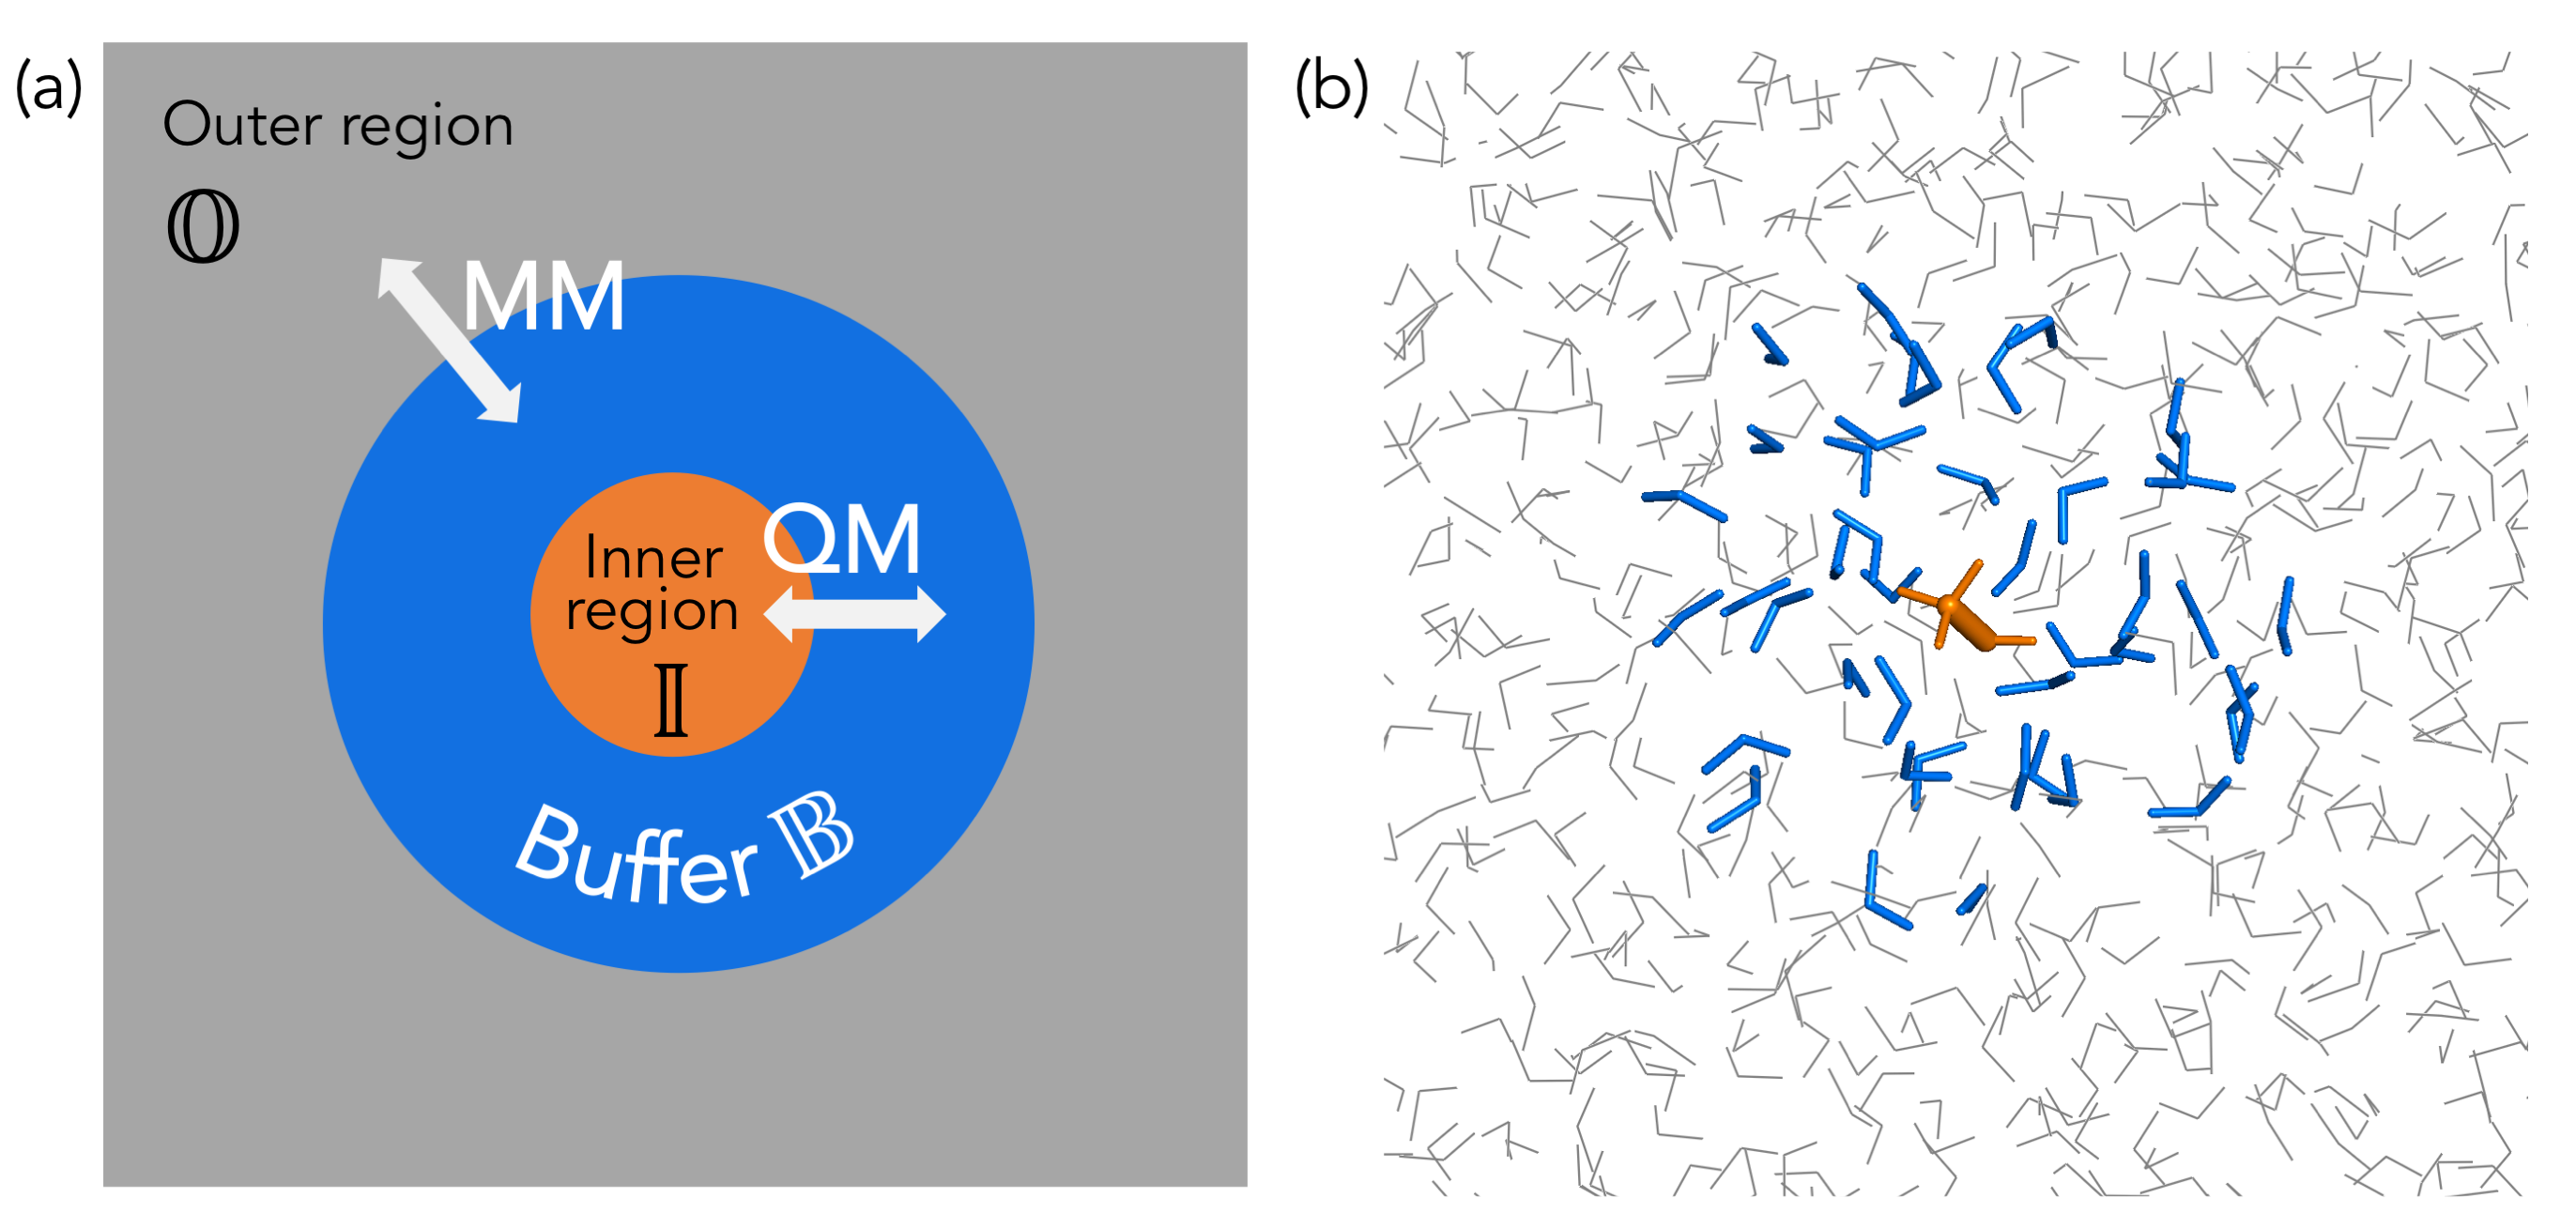
\includegraphics[scale=.33]{../09_tutorial_06/figures/BuRNN_scheme}
\caption{(a) BuRNN scheme with its three regions: Inner region (orange) described by quantum mechanics (QM), buffer region (blue) described by QM and molecular mechanics (MM), outer region (gray) described by MM. (b) Test system: methanol solvated in SPC water. Methanol therefore is the inner region, approximately two shells of water are the buffer region, the rest of the water box builds the outer region.}
\label{BuRNN_scheme}
\end{figure}


\subsubsection{Installation}
\paragraph{Prerequisites}
To compile and install GROMOS with the interface to SchNetPack (spk) to run NN models, you first need to have installed SchNetPack and the pybind11 library \cite{pybind11}. The interface uses the pybind11 library to call the model prediction functions in the Python code of SchNetPack. To install the SchNetPack and pybind11 library on your system, please follow their respective installation instructions. Tested version of SchNetPack is 1.0.0 and pybind11 v2.6.2.

\paragraph{GPU acceleration}
This part is optional to improve the efficiency of the simulations. The tasks in this tutorial are small enough to be run CPU-only in reasonable time. For the production runs this is inefficient since the training and evaluation of models on a GPU is usually many-folds faster. NN/MM MD simulations in GROMOS profit from this as well. Unfortunately, setting up your system to support the GPU acceleration is strongly architecture specific and is dependent on the installed CUDA and Pytorch versions. Please follow the installation instructions of CUDA and Pytorch to run tasks with the GPU acceleration.

\paragraph{GROMOS compilation}
Compilation of the NN-enabled version of GROMOS is activated by the \texttt{--enable-schnetpack} flag in the configuration step. The \texttt{configure} script looks up the pybind11 library automatically; however, based on the versions of the packages and the architecture, it might not be found. In that case you should provide the flags \texttt{PYFLAGS} and \texttt{PYLDFLAGS} to the \texttt{configure} script. The \texttt{PYFLAGS} variable holds the C preprocessor flags, which can be obtained by calling

\begin{lstlisting}[breaklines=true, breakatwhitespace=false]
python3 -m pybind11 --includes
\end{lstlisting}

The \texttt{PYLDFLAGS} are the linker flags. Depending on the Python version, they can be generated by calling either 

\begin{lstlisting}[breaklines=true, breakatwhitespace=false]
python3-config --ldflags
\end{lstlisting}

for Python <3.8, or 

\begin{lstlisting}[breaklines=true, breakatwhitespace=false]
python3-config --ldflags --embed
\end{lstlisting}

for newer versions. An example of the \texttt{configure} script then could be:
\begin{lstlisting}[breaklines=true, breakatwhitespace=false]
$ ./configure --enable-schnetpack PYFLAGS='-I/path/to/include/python3.7 -I/path/to/lib/python3.7/site-packages/pybind11/include' PYLDFLAGS='-L/path/to/lib/python3.7/config -L/path/to/lib -lpython3.7 -lcrypt -lpthread -ldl -lutil -lrt -lm'
\end{lstlisting}

Further steps follow the standard compilation:
\begin{lstlisting}[breaklines=true, breakatwhitespace=false]
$ make
$ make install
\end{lstlisting}


\subsubsection{Training dataset generation and model training}
The BuRNN approach replaces expensive QM calculations with NN predictions during MD simulations. In order to train NN models, QM data points for building a training data set have to be generated first. In this tutorial, an example QM data set has been generated using the semi-empirical program MOPAC \cite{Stewart1990MOPAC, Stewart2013MOPAC}. In practice, the choice of the QM software and the reference method to be used is entirely up to the user depending on the system and accuracy requirements. However, in order to prepare the training data set in a reasonable time, it is necessary to automate the QM calculations. In addition, it takes a certain amount of time to perform the QM calculations for all the snapshots generated by MD. Therefore, a small \href{https://github.com/LierB/gromos_tutorial_livecoms/tree/burnn_tutorial_rc/tutorial_files/t_06/train_dataset_tutorial/QM_dataset_example}{QM data set} has been prepared in advance for you (\texttt{train\_dataset\_tutorial/QM\_dataset\_example}). The entire process is described in the following section.


This tutorial will be accompanied by the \href{https://github.com/LierB/gromos_tutorial_livecoms/blob/burnn_tutorial_rc/tutorial_files/t_06/train_dataset_tutorial/tutorial_v2.ipynb}{jupyter notebook} (\texttt{train\_dataset\_tutorial/tutorial\_v2.ipynb}) to give you a hands-on example of building the training database. It will use the in-house written Python module \href{https://github.com/LierB/gromos_tutorial_livecoms/blob/burnn_tutorial_rc/tutorial_files/t_06/train_dataset_tutorial/additional_spk_utils.py}{\texttt{additional\_spk\_utils}} for building the training data set.


\paragraph{Extracting the QM regions from the MD trajectory}
The resulting QM data set will contain the inner plus buffer (IPB) region and the buffer region for each training configuration. Our protocol for creating such a data set is as follows: 
\begin{enumerate}
    \item Classical MD simulation of the system of interest.
    \item Extraction of the IPB regions from the MD trajectory.
    \item QM energy minimization for all (or selected) extracted IPB regions.
    \item Including all minimization steps into the data set.
    \item Extraction of the buffer regions from all the data points.
    \item Single-Point (SP) QM calculations for the IPB and buffer regions separately.
    \item Creation of the training database
\end{enumerate}


Classical MD simulations are performed as described in Tutorial 1. QM regions (inner + buffer regions) are extracted from each snapshot of the MD trajectory using the GROMOS++ program \texttt{filter}. The program writes out coordinate trajectories for atoms that are within a specified distance of a certain part of the system. The coordinates are all written into one \href{https://github.com/LierB/gromos_tutorial_livecoms/blob/burnn_tutorial_rc/tutorial_files/t_06/train_dataset_tutorial/filter/filter_output_example.cnf}{configuration file} (\texttt{filter\_output\_example.cnf}) in the \texttt{train\_dataset\_tutorial/filter} directory.

For methanol we specify all methanol atoms as filtering centers (\texttt{@atoms 1:a}) and filter with a chargegroup-based cut-off (\texttt{@pairlist CHARGEGROUP}) of 0.5 nm radius (\texttt{@cutoff 0.5}). The optimal/reasonable size for the buffer region can be determined from an rdf analysis. It should be as small as possible, as we want to save computational effort for the following QM calculations. The chargegroup cut-off scheme is important as we want to include full water molecules in the QM calculations. Then we extract individual QM regions into separated configuration files using an in-house written Python script. The arguments we use for \texttt{filter} are as follows:

\begin{lstlisting}[breaklines=true, breakatwhitespace=false]
@topo       path to the topology file
@pbc        r cog
@atoms      1:a
@pairlist   CHARGEGROUP
@cutoff     0.5
@outformat  cnf

@traj       path(s) to trajectory file(s)
\end{lstlisting}

We provide an example of two \href{https://github.com/LierB/gromos_tutorial_livecoms/tree/burnn_tutorial_rc/tutorial_files/t_06/train_dataset_tutorial/separated_cnf_files}{configuration files} (\texttt{train\_database\_tutorial/separated\_cnf\_files}) which will be further used in this tutorial. An example of the \href{https://github.com/LierB/gromos_tutorial_livecoms/blob/burnn_tutorial_rc/tutorial_files/t_06/train_dataset_tutorial/filter/filter_meoh_example.arg}{argument file} for \texttt{filter} is provided (\texttt{filter/filter\_meoh\_example.arg}).

\paragraph{QM calculations}
In this part we mainly focus on the concept of QM geometry optimization (GO) and single point calculations (SP) in the context of BuRNN. Once we have the coordinates of the IPB region, GO will optimize the atomic positions to find the local minimum of the QM potential energy surface. This calculation will not only find the local energy minimum but also connects the classical snapshots with the optimal QM conformations and thus represents a sufficient part of the conformational space of the system. Therefore we include all the optimization steps into the training dataset, but we have to be aware that the training dataset will be significantly increased in size. A lot of similar structures will be present at the end of the minimization and thus clustering before proceeding with the next step is recommended. We use MOPAC with the following keywords to perform the GO:

\begin{lstlisting}[breaklines=true, breakatwhitespace=false]
PM7 GRAD AUX(PRECISION = 9, XP, XS, XW) CHARGE=0
\end{lstlisting}

For each (remaining) optimization step, a single point (SP) QM calculation is required to receive the associated QM energy and gradients (forces). The SP calculation is not only done for the IPB region but also for the buffer region alone. The coordinates of the buffer region are identical for the two calculations. The number of atoms for the inner region is required, as these atoms need to be deleted for the second calculation (buffer region only). Furthermore, the geometry of water molecules in the buffer region has to be preserved as in the following BuRNN simulations the bonds will be constrained by the SHAKE algorithm \cite{RYCKAERT1977SHAKE}. The following MOPAC keywords are used for the SP calculations:

\begin{lstlisting}[breaklines=true, breakatwhitespace=false]
PM7 GRAD AUX(PRECISION = 9, XP, XS, XW) 1SCF CHARGE=0
\end{lstlisting}


The whole process of GO and subsequent SP calculations is automated by our Python module. The examples of the \href{https://github.com/LierB/gromos_tutorial_livecoms/tree/burnn_tutorial_rc/tutorial_files/t_06/train_dataset_tutorial/MOPAC_minimzation_files}{GO outputs} (\texttt{MOPAC\_minimzation\_files}) and \href{https://github.com/LierB/gromos_tutorial_livecoms/tree/burnn_tutorial_rc/tutorial_files/t_06/train_dataset_tutorial/QM_dataset_example}{SP outputs} (\texttt{QM\_dataset\_example}) are provided. GO was performed for two previously mentioned MD configurations. However, the size of the data set increased to 860 configurations after including the GO optimization steps.


\paragraph{Building a training database}
In this chapter we will explain how to build the ASE (atomic simulation environment) \cite{Larsen2017ASE} database from the previously calculated energies and forces of the snapshots. The procedure is described in more detail in the \href{https://github.com/LierB/gromos_tutorial_livecoms/blob/burnn_tutorial_rc/tutorial_files/t_06/train_dataset_tutorial/tutorial_v2.ipynb}{jupyter notebook}. The \texttt{additional\_spk\_utils} module will be used for storing the relevant properties and metadata in the ASE database. 


\paragraph{Model training}
The last step before running BuRNN simulations is the NN model training. In the previous parts, the ASE database was created based on structures from QM GO and SP calculations. We will now use SchNetPack for training of the example NN model. Due to the significant computational requirements of the NN model training we prepared fully trained \href{https://github.com/LierB/gromos_tutorial_livecoms/tree/burnn_tutorial_rc/tutorial_files/t_06/models}{NN models} in advance for you, which you can all find in the \texttt{models} directory. 


The SchNet model \cite{Schuett2018SchNet} is a convolutional neural network (CNN) with a continuous filter. It is very similar to the common CNNs used in image recognition. In contrast to images, molecules can not be described by the discrete matrix of pixels and thus the continuous filter is applied instead of a discrete one. The SchNet model is composed of two NNs. The main one is responsible for the prediction of the given property itself and uses the vector of atomic numbers for the given structure as an input. The second one generates the filter for the convolution using the atomic positions on the input. The main NN is divided into three blocks. The first is the embedding layer which creates the feature vectors for the individual atoms within the structure. Therefore the whole structure is represented by the 2D matrix of shape: number of atom-wise features \times number of atoms. The second part of the model is the series of the interaction blocks. One interaction block contains one convolutional layer. This block is responsible for creating the representation of the system. The last part is the output module which predicts the desired property of the structure, which is in our case the energy.

For the model training we use two scripts, the Python script \href{https://github.com/LierB/gromos_tutorial_livecoms/blob/burnn_tutorial_rc/tutorial_files/t_06/train_dataset_tutorial/spk_run.py}{\texttt{spk\_run.py}} and the bash script \href{https://github.com/LierB/gromos_tutorial_livecoms/blob/burnn_tutorial_rc/tutorial_files/t_06/train_dataset_tutorial/train.sh}{\texttt{train.sh}} which runs the Python script with all the specified arguments. The Python script loads the data from the previously prepared ASE database (the \texttt{datapath} variable) and splits it into a training, validation and test set. The split is controlled by the \texttt{--split} argument. We will use a split of 80/10/10\%. The NN model is built by fitting the hyperparameters. It is reasonable to use the default values to start with the training and then optimize them later. The number of atom-wise features and the number of interaction blocks are the most important hyperparameters of the SchNet architecture, as they define the model complexity and therefore the precision and computational costs. In our case we will train very small models with only a few features and interactions (arguments \texttt{features} and \texttt{interactions}), and we will train it only for two epochs (argument \texttt{n\_epochs}). The complete list of arguments (hyperparameters) for the \texttt{spk\_run.py} is listed in the \href{https://github.com/LierB/gromos_tutorial_livecoms/blob/burnn_tutorial_rc/tutorial_files/t_06/train_dataset_tutorial/tutorial_v2.ipynb}{jupyter notebook}. The following parameters are defined in our example training:
\begin{enumerate}
    \item[-] property = property to be predicted by the model (default energy)
    \item[-] derivative = derivative of the property to be predicted
    \item[-] rho = weight factor for the property and derivative, respectively
    \item[-] split = determines how many training, validation and test data will be selected, the first value for training data size, the second for validation data size, the rest of the dataset is used for the model evaluation (default (None, None))
    \item[-] batch\_size = batch size (default 8)
    \item[-] n\_epochs = maximum number of training epochs (default 5000)
    \item[-] lr = learning rate (default 0.0001)
    \item[-] lr\_patience = learning rate will be decreased after the certain number of epochs without improvement of the model (default 25)
    \item[-] lr\_min = minimal learning rate, when the value is reached, the training process is stopped (default 1e-06)
    \item[-] cutoff = cutoff for long-range interactions (default 5.0)
    \item[-] num\_gaussians = number of gaussians to describe (default 50)
    \item[-] features = number of atom-wise features (default 128)
    \item[-] interactions = number of interaction blocks (default 3)
\end{enumerate}


The main goal of the training is to obtain a potential energy function, that is as close as possible to the reference one. Since beside the energies, we also have the analytical gradients, or negative forces, it is beneficial to provide them for the training as well. They carry the essential information about the shape of the function at the provided data points, which significantly improves the accuracy of the generated model. For that purpose, Schnetpack has a built-in functionality, which uses a loss function combining energies and forces. A loss weight (the argument \texttt{--rho}) is introduced to control the trade-off between the energy loss and the force loss. In this tutorial, we provide the optimized weights of 0.01 for the energies and 0.99 for the gradients. Please note, that the loss function mixes units of energies and forces and therefore the weights are unit-dependent. The gradients are not trained as a separate property; instead, they are used to improve the true analytical gradients of the model. In production runs, the model then provides the analytical gradients, which is essential for the conservation of energy in MD simulations.

The \texttt{train.sh} bash script, which calls the Python script for training, is written as follows:
\begin{lstlisting}[breaklines=true, breakatwhitespace=false]
#!/bin/bash

datapath= your path to the ASE database
modelpath= your path where the model will be stored

# model training
python spk_run.py train schnet custom $datapath $modelpath --property energy --derivative forces --rho property=0.01 derivative=0.99 --split 688 86 --batch_size 8 --n_epochs 2 --lr 0.0001 --lr_patience 10 --lr_min 1e-06 --cutoff 100.0 --num_gaussians 50 --features 32 --interactions 1
\end{lstlisting}


The script also calls the \texttt{spk\_run.py} in the evaluation mode which evaluates the model against the test data:

\begin{lstlisting}[breaklines=true, breakatwhitespace=false]
# model evaluation
python spk_run.py eval $datapath $modelpath --split test --batch_size 1
\end{lstlisting}


Run the script to train and evaluate the example model:

\begin{lstlisting}[breaklines=true, breakatwhitespace=false]
$ ./train.sh
\end{lstlisting}


The training will produce several files in the model-path directory. The model, the evaluation file, a training log file, a file with the random split, a checkpoint file and a json file with the model settings. The checkpoint file is written periodically and can be used to restart the training. For BuRNN simulations, we need to train two NN models, as we use the second model to evaluate the predictions of the first model.



\subsubsection{BuRNN simulation}

For the BuRNN simulation, we have to specify, which atoms are in the QM and buffer regions. GROMOS allows for adaptive buffer region, i.e. the atoms are allowed to move freely between the MM and buffer region. The atoms of the QM region are not allowed to change. This information together with other specifications are specified in an additional input file \href{https://github.com/LierB/gromos_tutorial_livecoms/blob/burnn_tutorial_rc/tutorial_files/t_06/md_burnn/meoh.qmm}{\texttt{meoh.qmm}} in the \texttt{md\_burnn} directory:

\begin{lstlisting}[breaklines=true, breakatwhitespace=false]
TITLE
qmmm specification file for BuRNN  
END
QMUNIT
# QMULEN    QMUENE    QMUFOR    QMUCHR
     0.1     4.184    -41.84       1.0
END
\end{lstlisting}

The \texttt{QMUNIT} block may convert units of the model by a conversion factor for distances (\texttt{QMULEN}), energies (\texttt{QMUENE}), forces (\texttt{QMUFOR}), and charges(\texttt{QMUCHR}).

\begin{lstlisting}[breaklines=true, breakatwhitespace=false]
NNDEVICE
auto
END
NNMODEL
/path/to/best_model
# MT LT
   0  1
END
NNVALID
/path/to/best_model2
# NUMSTP THRSH FCON 
       1 4.184  0.0
END
\end{lstlisting}


The \texttt{NNDEVICE} block specifies the architecture for model execution. Allowed options are \texttt{auto}, \texttt{cuda} or \texttt{cpu}. Selecting \texttt{auto} instructs to run on GPU if available, or else fall back to CPU.

In the next block, \texttt{NNMODEL}, the path to the prediction model is specified. The model type (\texttt{MT}) is set to 0, meaning that BuRNN will be run with a single NN evaluation on the previously trained energy differences. It would also be possible to calculate differences just during the simulation in a combined model or even calculate it with QM on the fly by setting it to 1. The learning type (\texttt{LT}) is set to 1 for a standard calculation. 

The \texttt{NNVALID} block is optional and used if a second (validation) model is evaluated during the simulation. In this case, we use a validation model which also predicts the energy of the given configuration. The predictions of the two individually trained models are compared to estimate the robustness of the prediction. The models have to be trained with the same hyperparameters on the same data set, but with a different random split.

The models will be compared at every nth step (\texttt{NUMSTP}), and the energy difference will be deemed accurate if it is below the threshold (\texttt{THRSH}). If it is above the threshold, the force constant (\texttt{FCON}) can be set positive, to push back the atoms to a configuration with a better agreement between the models. 

We set the threshold to 4.184 kJ/mol, which reflects the chemical accuracy of 1 kcal/mol. The difference between the models are calculated at each time step (\texttt{NUMSTP=1}). This can be easily changed if we need to generate coordinates that are not included in the training set or if the simulation is not stable yet. Once we have a stable simulation, we can e.g. check the differences only every 100th step.

\begin{lstlisting}[breaklines=true, breakatwhitespace=false]
QMZONE
# CHG MULT
    0    1
# RESIDUE   ATOM     QMI   QMZ   QMLI
   1 MeOH   CA         1     6      0
   1 MeOH   OB         2     8      0
   1 MeOH   HA1        3     1      0
   1 MeOH   HA2        4     1      0
   1 MeOH   HA3        5     1      0
   1 MeOH   HB1        6     1      0
END
BUFFERZONE
# CHG MULT CUTOFF 
    0    1    0.5
# RESIDUE   ATOM     QMI   QMZ   QMLI
   1 SOLV   OW         7     8     0
   1 SOLV   HW1        8     1     0
   1 SOLV   HW2        9     1     0
   2 SOLV   OW        10     8     0
   2 SOLV   HW1       11     1     0
   2 SOLV   HW2       12     1     0
   ...
END
\end{lstlisting}


These blocks finally contain the atoms that belong to the inner region (\texttt{QMZONE}) and that are allowed to be a part of the buffer region (\texttt{BUFFERZONE}). In the first line of both blocks we specify the charge and multiplicity of the given zone. In the \texttt{BUFFERZONE} block we also define the cutoff which we choose to be 0.5 nm. The atoms specified in the \texttt{BUFFERZONE} block are considered as buffer region as soon as they come within the cutoff of any atom of the inner region.

In addition to the separate input file, the \href{https://github.com/LierB/gromos_tutorial_livecoms/blob/burnn_tutorial_rc/tutorial_files/t_06/md_burnn/md.imd}{\texttt{md.imd}} file requires a \texttt{QMMM} block:
\begin{lstlisting}[breaklines=true, breakatwhitespace=false]
QMMM
# NTQMMM NTQMSW RCUTQM NTWQMMM QMLJ QMCON      
 MMSCALE
       1      5    1.4       0    0     0
    -1.0
END
\end{lstlisting}

Most of the parameters are only relevant for conventional QM/MM simulations and will therefore not be explained in detail.

QM/MM hybrid simulations (with mechanical embedding) are enabled by setting the first parameter \texttt{NTQMMM=1}. The interactions between the inner region and the outer region are essentially on the mechanical embedding level. \texttt{NTQMSW} determines which software will be used for the QM calculation. The SchNetPack corresponds to \texttt{NTQMSW=5}. The cutoff determined by \texttt{RCUTQM} is only relevant for electrostatic or polarizable embeddings and for \texttt{NTQMMM=1} it is ignored. \texttt{NTWQMMM} can be used if QM/MM related data should be written to a separate trajectory every n-th step. For BuRNN simulations we do not want to calculate LJ between QM atoms \texttt{QMLJ=0}. Constraining the bond lengths in the QM zone is optional (\texttt{QMCON}). With \texttt{MMSCALE} we can scale MM charges (by a scaling factor), but if \texttt{MMSCALE<0} no scaling is applied.

In analogy to Tutorial 1 job scripts can be generated with the \textt{mk\_script} program. The argument file \href{https://github.com/LierB/gromos_tutorial_livecoms/blob/burnn_tutorial_rc/tutorial_files/t_06/md_burnn/md_mk_script.arg}{\texttt{md\_mk\_script.arg}} is also provided for you. Finally, you can execute the run files.


\subsubsection{BuRNN (example) analysis}
The trajectory files produced by the BuRNN simulation are the same as those produced by the standard MD simulation in GROMOS, meaning that we can perform any analysis. Here we decided to show hydrogen bonds and the radial distribution function (rdf) between the methanol treated at the QM level and the MM water molecules around. The argument files \href{https://github.com/LierB/gromos_tutorial_livecoms/blob/burnn_tutorial_rc/tutorial_files/t_06/md_burnn/ana/hbond/hbond_meoh.arg}{\texttt{hbond\_meoh.arg}} and \href{https://github.com/LierB/gromos_tutorial_livecoms/blob/burnn_tutorial_rc/tutorial_files/t_06/md_burnn/ana/rdf/rdf_ob_ow.arg}{\texttt{rdf\_ob\_ow.arg}} for the GROMOS programs \texttt{hbond} and \texttt{rdf} are provided in the \texttt{ana} directory. 
The results can be seen in Figure~\ref{BuRNN_ana}.

\begin{figure}[H]
\centering
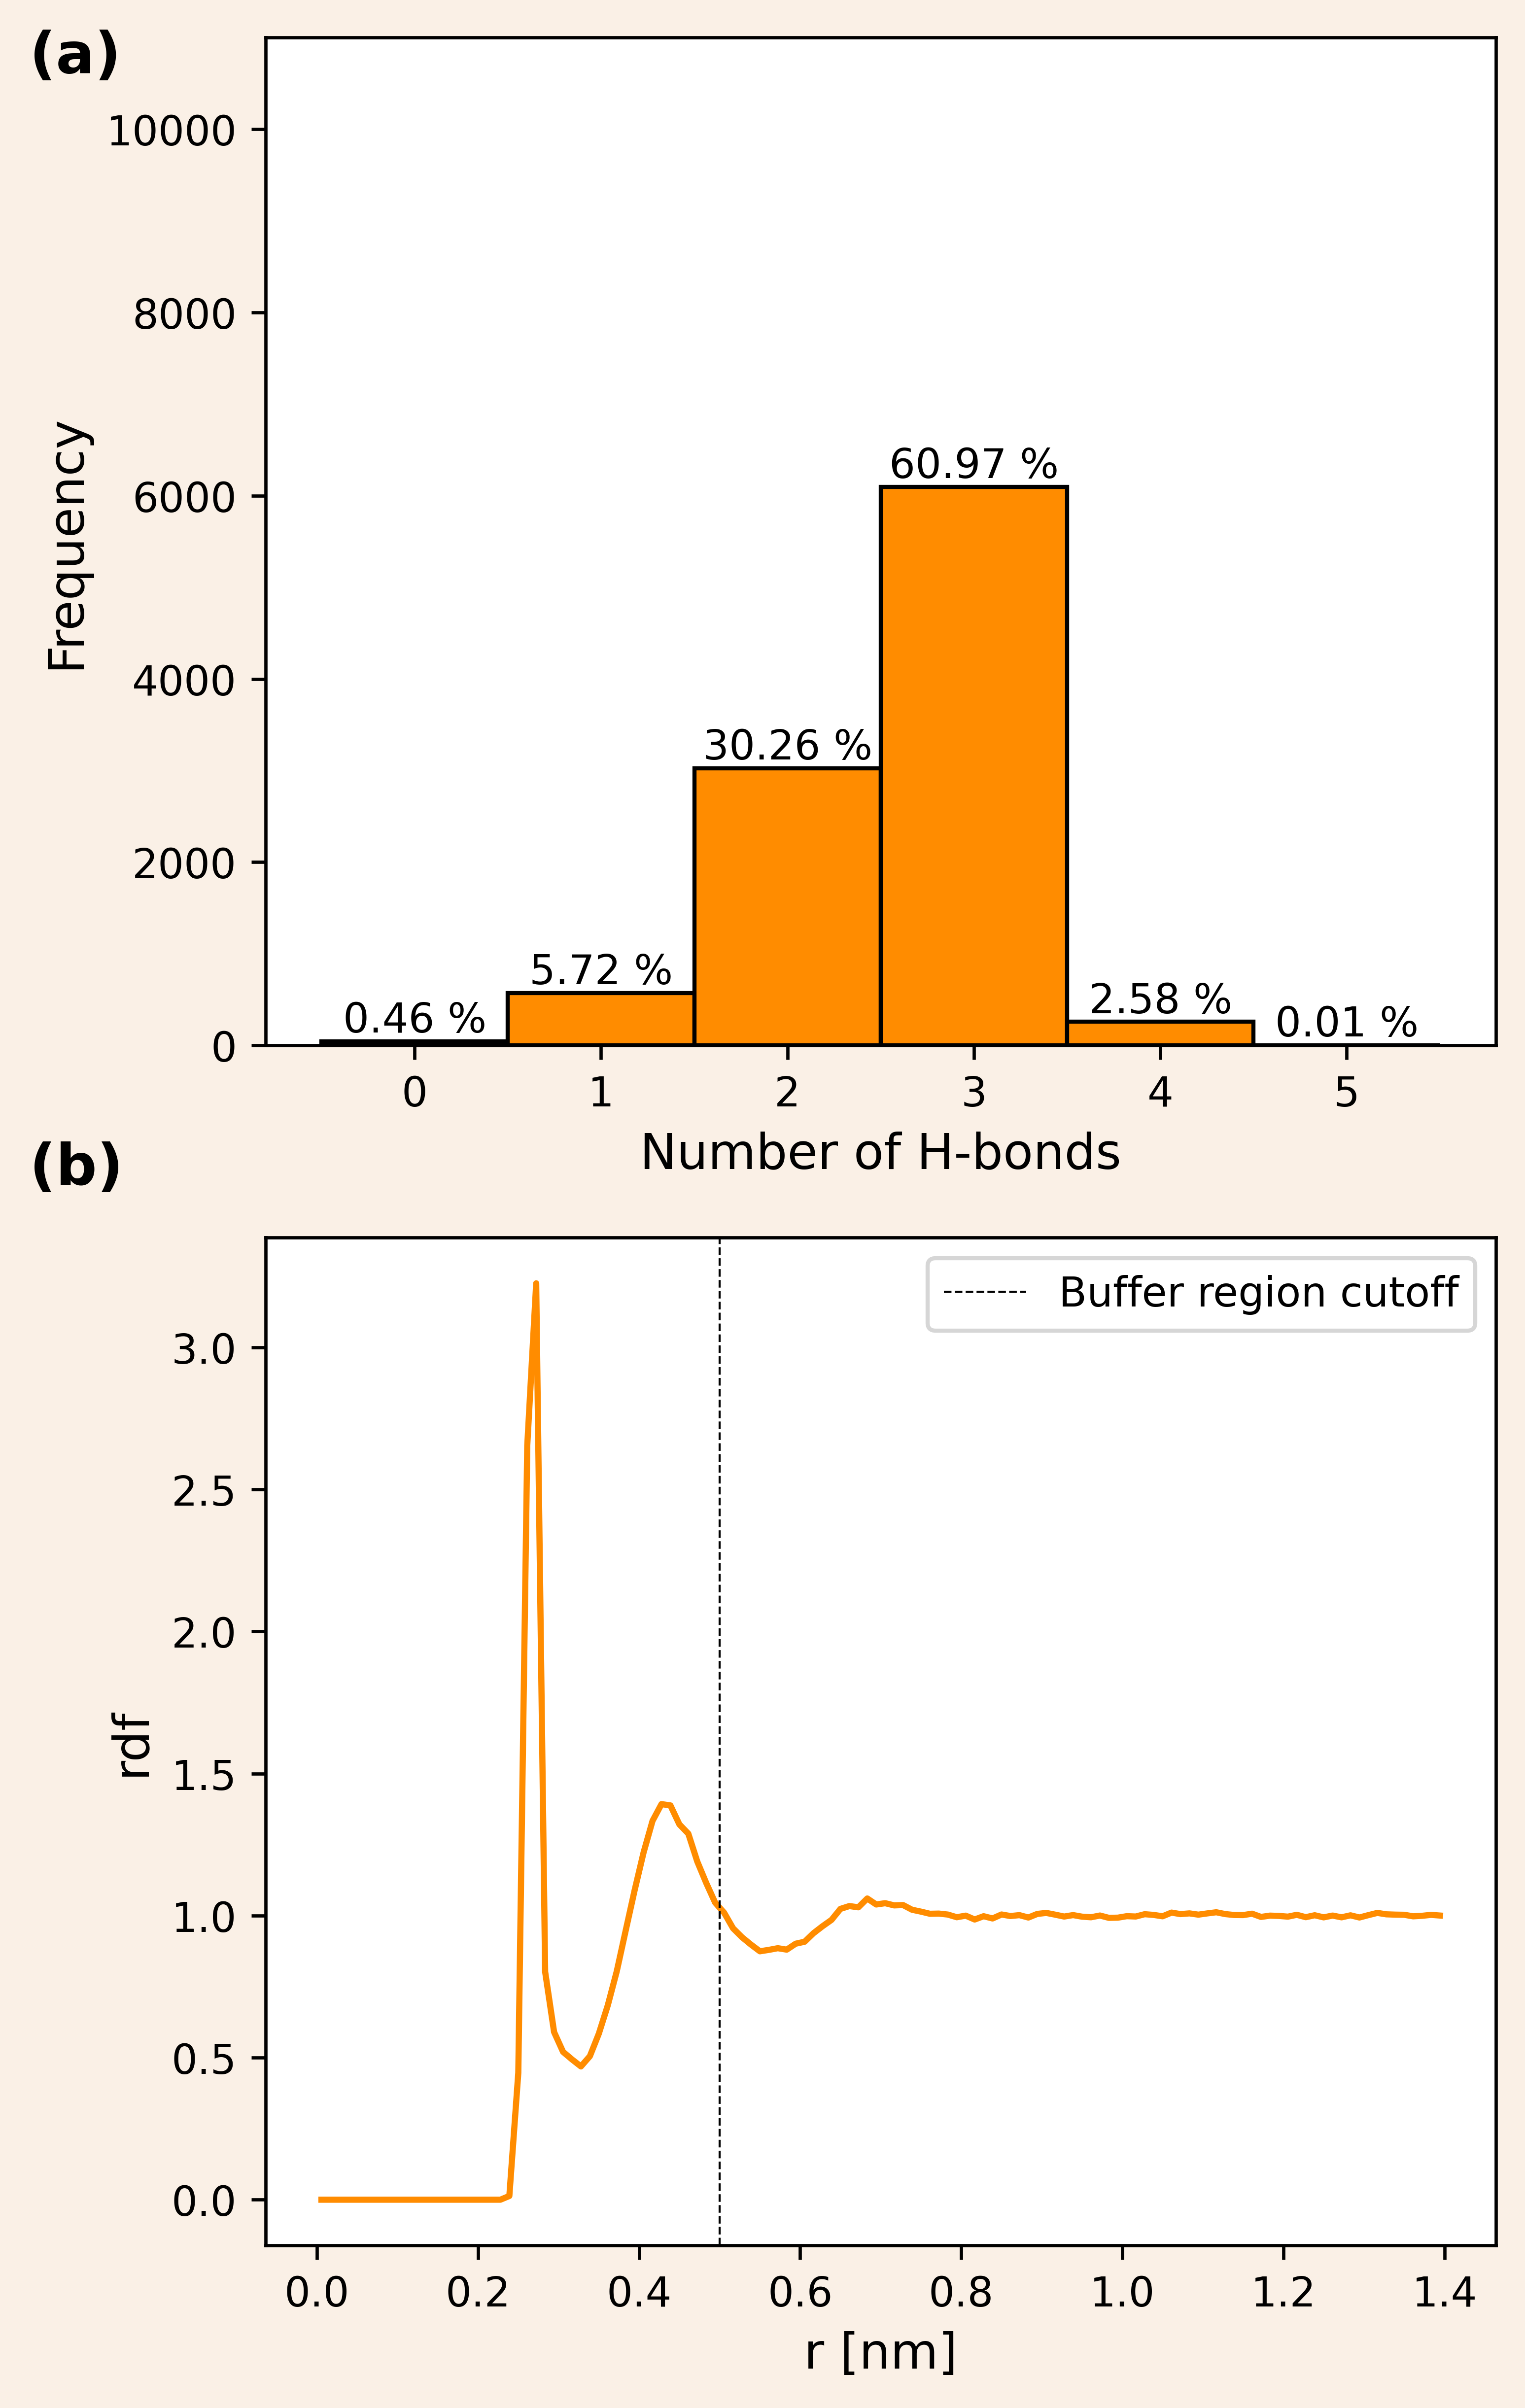
\includegraphics[scale=.66]{../09_tutorial_06/figures/BuRNN_ana.png}
\caption{\textbf{BuRNN simulation analysis. (a)} The number of hydrogen bonds formed between methanol and water for each snapshot of the trajectory. \textbf{(b)} Radial distribution function between the methanol's oxygen and all the oxygen atoms of the water molecules. The results are based on a 2 ns BuRNN simulation of the methanol on water.}
\label{BuRNN_ana}
\end{figure}



\subsubsection{Advanced options}
\paragraph{Charge model}
For running BuRNN simulations with dynamic QM charges, charges first need to be calculated with the QM method of choice and included in the training dataset. A separate NN has to be trained for the charges. SchNet was therefore adapted and the version can be found in \href{https://github.com/juliawestermayr/schnetpack}{this repository}.
In the \texttt{charge.qmm} file the \texttt{NNCHARGE} block has to be added. 

\begin{lstlisting}[breaklines=true, breakatwhitespace=false]
NNCHARGE
/path/to/best/charge_model
# NUMSTP
       1
END
\end{lstlisting}

This block contains the path to the NN charge model and at which nth step (\texttt{NUMSTP}) the charges should be updated.

Including a charge model was e.g. relevant for the hexa-aqua iron, the model system of the original BuRNN paper \cite{Lier2022BuRNN}.

%\paragraph{Adaptive sampling}
